\section{Contact diameters}

The ''contact diameter'', $\sigma_{ij}$ has been mentioned several times thus far, and has been taken to be some distance in the range of the particle sizes. In the case of additive hard spheres, the contact diameter can unambiguously be defined as the distance between the centre of mass of the two particles at contact. However, for Mie particles this definition is not equally straight forward. In this section, various ways of defining the contact diameter, and the inherent underlying assumptions behind the different definitions will be discussed.

Firstly, it is worth mentioning that applying the multicomponent, density corrected solutions proposed by de Haro et al. to Mie fluids implies the assumption that the contact diameters are independent of particle velocities at collision. This assumption is necessary due to the fact that the integral of Equation \eqref{eq:streaming_op} is one over the velocity space. The contact diameters are permitted to be functions of the temperature, and thereby the mean velocities, as well as density and composition but must be constant for all particles in a given state.

One could, in principle, define the contact diameters as some function of the velocities, but this would severely limit the possibility of utilising previously obtained results from the literature. Therefore, such an approach has not been attempted here.

When defining the contact diameters of Mie particles, we note the two roles this distance plays. The first is describing the covolume of the mixture, and the modified probability of finding two particles at contact through the radial distribution function ''at contact''. The second is describing the instantaneous transfer of energy and momentum from one particle to the other when particles collide. This effect manifests itself as the second terms in the expressions for the conductivity and viscosity, which depends on the density, contact diameters and rdf. but not on the polynomial expansion coefficients. Because the contact diameter plays two distinctly different roles, it is not necessarily so that the length one should use in these two roles must be the same.

To evaluate the radial distribution function ''at contact'' a highly convenient choice of the contact diameter is the Mie parameter $\sigma_{ij}$. This allows one to directly apply the expressions proposed by Lafitte et al. for the rdf. at contact.\cite{lafitte2013accurate} This formulation of the rdf. at contact has been shown to give accurate predictions of thermodynamic properties of fluids, and the associated distance is therefore likely to give a good representation of the covolume of the mixture. Therefore, it is believed that using $\sigma_{ij}$ as the contact diameter when computing the rdf. at contact is not only a convenient choice, but also a choice that allows accurate representation of the modified probability of contact between particles due to volume exclusion.

Regarding the second property described by the contact diameter, the instantaneous transfer of energy and momentum at the moment of collision, a distance more directly related to the collision dynamics was chosen. Firstly, note that the equilibrium vdf. given in Equation \eqref{eq:eq_vdf} does not depend on the contact diameters. We regard a colliding pair of particles, and define the contact diameter as the average distance of closest approach ($R$) during collision where the particles repel each other (e.g. collisions where $\theta < \frac{\pi}{2}$). Further, we compute this average for a mixture at equilibrium, when $f_i = f_i^{(0)}$. The contact diameter is then given by

\begin{equation}
    \Bar{R}_{ij} = \int_{0}^{\infty} \int_0^{b'} R_{ij}(g_{ij}, b) \d b \d g_{ij}
    \label{eq:R_defl}
\end{equation}

where $g_{ij}$ is the relative speed of the colliding pair and $b'$ is the solution to the equation

\begin{equation}
    \theta_{ij}(b'; g_{ij}) = 0.
\end{equation}

This integral is somewhat computationally expensive to evaluate, but may be simplified by noting that $R(g_{ij}; b)$ is reasonably symmetric about $g = \Bar{g}$, the average relative speed, as shown in Figure \ref{fig:symmetry_closest_appr}. Due to this symmetry, a good approximation to the integral of Equation \eqref{eq:R_defl} is given by

\begin{equation}
    \Bar{R}_{ij} = \int_0^{\Bar{b}'} R_{ij}(b; \Bar{g}_{ij}) \d b
\end{equation}
with $\Bar{b}'$ given by
\begin{equation}
    \theta_{ij}(\Bar{b}'; \Bar{g}_{ij}) = 0.
\end{equation}

\begin{figure}[htb]
    \centering
    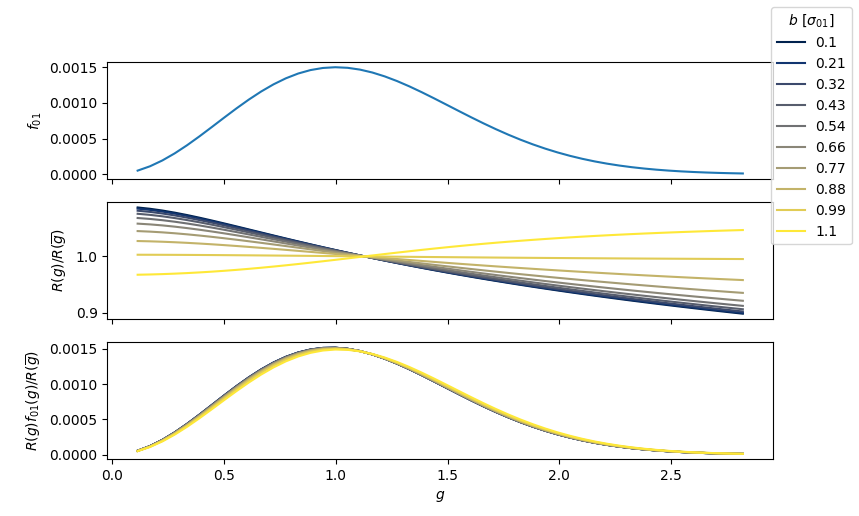
\includegraphics[width=\textwidth]{symmetry_closest_appr.png}
    \caption{The distance of closest approach as a function of dimensionless relative velocity $g$ and impact parameter $b$ at $T = \SI{500}{\kelvin}$}
    \label{fig:symmetry_closest_appr}
\end{figure}

This integral was evaluated using a six-point Gauss-Legendre quadrature, after investigating the convergence behaviour of the quadrature and finding that this was sufficient to achieve a relative precision of $\approx 10^{-8}$.